% Created 2017-03-24 Fri 11:09
\documentclass[10pt,t,a4paper]{beamer}
\usepackage[utf8]{inputenc}
\usepackage[T1]{fontenc}
\usepackage{fixltx2e}
\usepackage{graphicx}
\usepackage{longtable}
\usepackage{float}
\usepackage{wrapfig}
\usepackage{rotating}
\usepackage[normalem]{ulem}
\usepackage{amsmath}
\usepackage{textcomp}
\usepackage{marvosym}
\usepackage{wasysym}
\usepackage{amssymb}
\usepackage{hyperref}
\tolerance=1000
\usetheme{BTH_msv}
\author{Mikael Svahnberg\thanks{Mikael.Svahnberg@bth.se}}
\date{2017-03-23}
\title{User Stories \\\\ and Use Cases}
\hypersetup{
  pdfkeywords={},
  pdfsubject={},
  pdfcreator={Emacs 25.1.1 (Org mode 8.2.10)}}
\begin{document}

\maketitle

\section{Classroom}
\label{sec-1}
\begin{frame}[label=sec-1-1]{User Stories}
\begin{itemize}
\item User Stories are the currently preferred way in agile of writing requirements.
\item Simpler structure than the ``regular'' requirements
\item Not usually worked with in lenghty documents
\begin{itemize}
\item Rather, just enough to fill a sprint
\end{itemize}
\item Template: \emph{As a <type of user> I want <some goal> so that <some reason>.}
\end{itemize}
\end{frame}
\begin{frame}[label=sec-1-2]{User Stories Examples}
\begin{quote}
\begin{itemize}
\item As a software designer I want to document what the customer is telling me so that I can discuss my understanding of their requirements with them.
\item As a software designer I want to document what the customer is telling me so that I can easily continue designing based on a joint understanding.
\item As a software designer I want to be able to reuse common procedures between my use cases so that I only have to maintain them in one place.
\item As a project manager I need to decide what to focus on building right now so that I best satisfy all customers' expectations.
\item As a product manager I want to make sure that we are building software of high quality.
\end{itemize}
\end{quote}
\end{frame}
\begin{frame}[label=sec-1-3]{Discuss: Good and Bad Requirements I}
Users shall be able to view a personal calendar and recent notifications in the system.

\begin{verse}
Use Case: View Calendar and Notifications \\
Actors: System Users \\
Description: \\
\hspace*{2em}A user requests to view their personal calendar. \\
\hspace*{4em}The system displays the users' personal calendar. \\
\hspace*{2em}A user requests to view their recent notifications. \\
\hspace*{4em}The system displays the users' recent notifications. \\
\end{verse}

\only<2>{
As a regular user I want to be able to view my personal calendar and recent notifications \emph{so that I can make sure that a new notification does not double-book me on an event}.
}
\end{frame}
\begin{frame}[label=sec-1-4]{User Stories and UML Use Cases}
\begin{itemize}
\item User Stories are \emph{not} UML Use Cases.
\begin{itemize}
\item $\ldots$ But you can use them as a starting point (for the Description)
\item \alert{Discuss:} Why are they not the same? Why do we need both?
\end{itemize}
\item User Stories have ``Conditions of Satisfaction'' -- Acceptance criteria.
\begin{itemize}
\item Where would you fit these in a Use Case?
\item \emph{Would} you fit these in a Use Case?
\end{itemize}
\end{itemize}

\begin{block}{Value}
\begin{itemize}
\item Both User Stories and UML Use Cases focus on \emph{value}.
\item They describe something that adds value to the system.
\begin{itemize}
\item e.g. A Business Process
\end{itemize}
\end{itemize}
\end{block}
\end{frame}
\begin{frame}[label=sec-1-5]{UML Use Cases}
\begin{itemize}
\item A concrete scenario
\item Normally describes a process consisting of some back-and-forth interaction with the system.
\item A collection of requirements, working together to solve a particular scenario.
\item Focus primarily on the \emph{positive} scenario
\begin{itemize}
\item everything goes as expected.
\end{itemize}
\item Describes a particular instance of the scenario
\begin{itemize}
\item not all possible cases.
\end{itemize}
\end{itemize}
\end{frame}
\begin{frame}[shrink=15,label=sec-1-6]{UML Use Cases}

\begin{itemize}
\item Name
\item Actors
\item Brief Description
\end{itemize}

\begin{verse}
Use Case: Return Book \\
Actors: Customer, Librarian \\
Description: A customer returns a book. The librarian scans the barcode and the system registers the book as being back in the library. \\
\end{verse}

\begin{block}{Discuss}
\begin{itemize}
\item Why can't the customer scan the barcode themselves?
\item Why barcode?
\item Why does the system need to know that the book is back in the library?
\item How do we test this?
\begin{itemize}
\item How do we regression test this?
\end{itemize}
\item From a Requirements Engineering perspective, how can we find more information if we need it?
\end{itemize}
\end{block}
\end{frame}
\begin{frame}[label=sec-1-7]{Expanded Use Cases}
\begin{verse}
Use Case: name \\
Actors: primary actors \\
Description: brief description \\
Main Course of Events: \\
\end{verse}
\begin{center}
\begin{tabular}{ll}
Actor & System\\
\hline
1. action & 2. response\\
… & …\\
n-1. action & n. response\\
\end{tabular}
\end{center}

\begin{verse}
Alternative Flow of Events: \\
\hspace*{3em}p. a description of what might happen instead, and how the system reacts to this. \\
\end{verse}
\end{frame}
\begin{frame}[label=sec-1-8]{Discussion: What's in a Name}
What are good names for use cases?

\begin{block}{Example: Discussion Forum}
What are the primary use cases for a discussion forum?
\end{block}
\end{frame}
\begin{frame}[label=sec-1-9]{Planning with the help of Use Cases}
\begin{itemize}
\item Use Cases describe high-level usage scenarios
\begin{itemize}
\item features?
\end{itemize}
\item Which use case should be implemented first?
\item Which use cases contribute to a Minimum Viable Product?
\end{itemize}
\end{frame}
\begin{frame}[label=sec-1-10]{Discussion on Use Case Ranking}
\begin{block}{Increase ranking of a use case if it}
\begin{itemize}
\item has direct impact on architectural design
\begin{itemize}
\item example: adds classes to domain layer, require persistent services
\end{itemize}
\item includes risky, time-critical, complex functions
\item involves new research or technology
\item represents primary business processes
\item directly supports revenue or decreased costs
\end{itemize}
\end{block}
\begin{block}{Discuss}
For each of these cases, why does it increase the rank of a use case?
\end{block}
\end{frame}

\begin{frame}[label=sec-1-11]{Use Case Ranking Techniques}
\begin{itemize}
\item Scored (Numerical Weights)
\item Discrete (High, Medium, Low)
\item Simple Ordering (bubble sort?)
\item MoSCoW (Must have, Should have, Could have, Won't have)
\item Cumulative Voting
\end{itemize}
\end{frame}
\begin{frame}[label=sec-1-12]{Use Case Diagrams}
\begin{itemize}
\item Overview of Use Cases, System Boundaries, and Actors
\end{itemize}

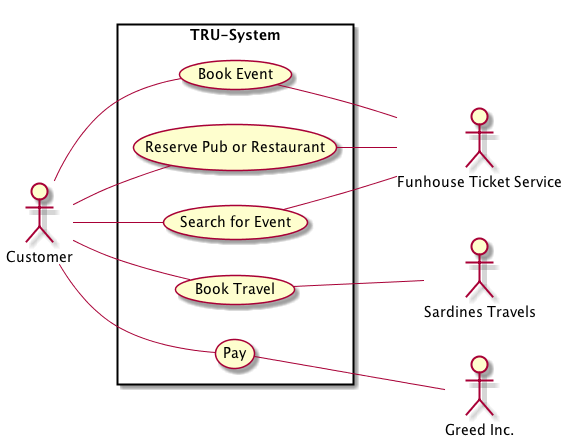
\includegraphics[height=5cm]{FUCD.png}     
\end{frame}
\begin{frame}[label=sec-1-13]{Use Case Reuse}
\begin{itemize}
\item Extend and Include
\item \alert{Do this later!} Your main job is still to understand \emph{what} the customer wants. Relating use cases is mostly a modelling exercise.
\end{itemize}

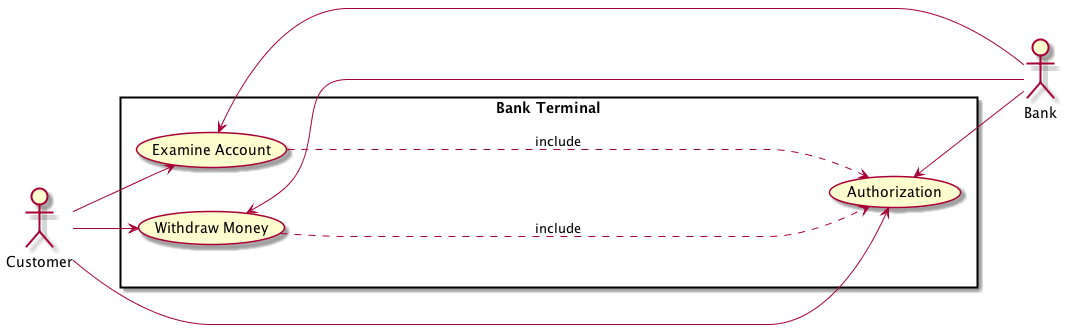
\includegraphics[width=.9\linewidth]{FStructuringUC1.png}
\end{frame}

\begin{frame}[fragile,shrink=40,label=sec-1-14]{Use Case \texttt{WithdrawMoney}}

 \begin{verse}
Use Case: Withdraw Money \\
Primary Actor: Customer \\
Actors: Bank \\
\vspace*{1em}
Description: A customer authenticates themselves against the bank, and selects \\
\hspace*{2em}how much money they want to withdraw and in what types of banknotes. The system \\
\hspace*{2em}updates the account (if there is enough money) and gives the money to the customer. \\
\vspace*{1em}
Main Flow of Events: \\
\end{verse}
\begin{center}
\begin{tabular}{ll}
Actor & System\\
\hline
1. Customer \emph{Authorises} themself to the machine & 2. Initiate use case \uline{Authorisation}\\
3. Customer \emph{Checks} how much money is available & 4. System displays the amount of money on the account.\\
5. Customer decides how much money they want & \\
6. Customer decides what banknotes they want & 7. System verifies that there are sufficient funds in the account.\\
 & 8. System subtracts desired amount from account.\\
 & 9. System dispenses money (according to the preferred banknotes).\\
 & 10. System returns card.\\
\hline
\end{tabular}
\end{center}
\end{frame}
\begin{frame}[fragile,shrink=15,label=sec-1-15]{Use Case \texttt{WithdrawMoney}}

 \begin{verse}
Use Case: Withdraw Money \\
Primary Actor: Customer \\
Actors: Bank \\
\vspace*{1em}
Preconditions: \\
- Customer is a customer at the bank \\
- There is money in the bank terminal \\
\vspace*{1em}
Postconditions: \\
- Customer walks away with cash in hand \\
- The customers account is accordingly updated \\
\vspace*{1em}
Description: A customer authenticates themselves against the bank, and selects \\
\hspace*{2em}how much money they want to withdraw and in what types of banknotes. The system \\
\hspace*{2em}updates the account (if there is enough money) and gives the money to the customer. \\
\vspace*{1em}
Main Flow of Events: \\
\end{verse}
\begin{center}
\begin{tabular}{ll}
Actor & System\\
\hline
1. Customer \emph{Authorises} themself to the machine & 2. Initiate use case \uline{Authorisation}\\
3. Customer \emph{Checks} how much money is available & 4. System displays the amount of money on the account.\\
5. Customer decides how much money they want & \\
6. Customer decides what banknotes they want & 7. System verifies that there are sufficient funds in the account.\\
 & 8. System subtracts desired amount from account.\\
 & 9. System dispenses money (according to the preferred banknotes).\\
 & 10. System returns card.\\
\hline
\end{tabular}
\end{center}
\begin{verse}
Alternative Flows: \\
\hspace*{1em}- 2. Customer fails to authorise themselves correctly. The transaction is aborted. \\
\hspace*{1em}- 7. There are not enough money in the account. The transaction is aborted and an error message is shown. \\
\hspace*{1em}- 9. The desired banknotes are not available. The system dispenses other banknotes. \\
\hspace*{1em}- 9. There is not enough money in the machine. The transaction is aborted and the system initiates the \uline{out of money} use case. \\
\vspace*{1em}
\end{verse}
\end{frame}
\begin{frame}[label=sec-1-16]{Extends vs Includes}
\begin{itemize}
\item Extends $\approx$ inheritance: Your new use case is the same as the old, \emph{except} for any modifications you introduce.
\item Includes ``borrows'' a separate use case and inserts it into the flow of the current use case.
\item In fact, you may use the \emph{include} relationship to compose smaller scenarios into a bigger one.
\end{itemize}

\begin{block}{Example}
\begin{itemize}
\item Example the use case ``Pay for Items'' can \emph{include} ``Pay by cash'', ``Pay by card'', and ``Pay by cheque''.
\item The use case ``Pay with Gift Certificate'' \emph{extends} ``Pay by cash''.
\end{itemize}
\end{block}
\end{frame}
\begin{frame}[label=sec-1-17]{Extends vs Includes}
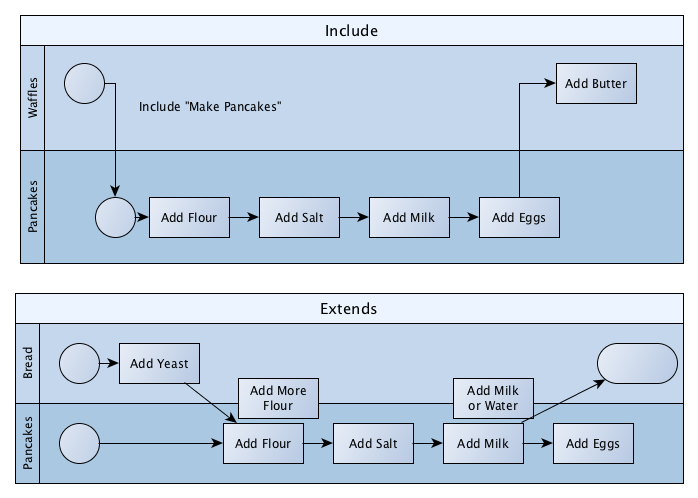
\includegraphics[height=6cm]{./IUseCaseIncludevsExtend.png}
\end{frame}
% Emacs 25.1.1 (Org mode 8.2.10)
\end{document}